\chapter{Algorithms: Search}

\section{Linear Search Algorithm \cite{gfg-linear-search}}\label{Linear Search Algorithm}

\begin{table}[h]
    \begin{minipage}[t]{0.5\linewidth}
        \begin{figure}[H]
            \centering
            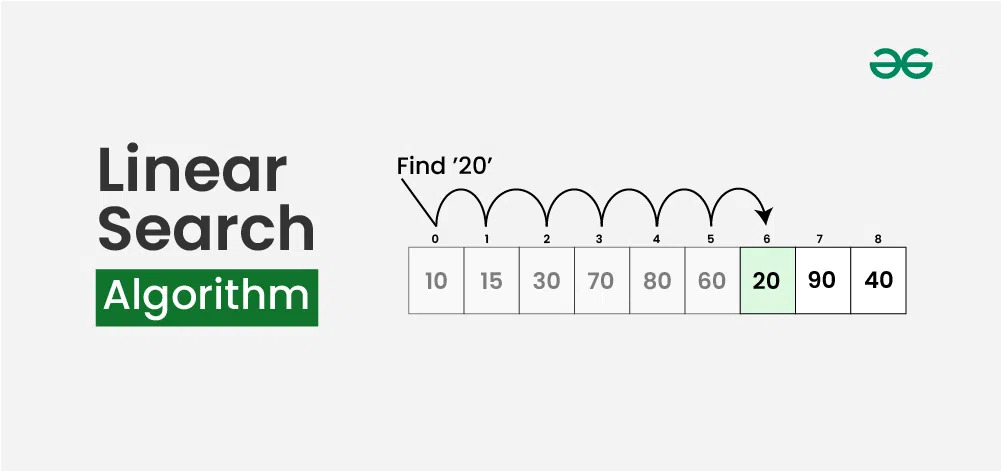
\includegraphics[width=\linewidth,height=6cm,keepaspectratio]{Pictures/ds-algo/Linear-Search-algorithm.jpg}
            \caption{Linear Search Algorithm}
        \end{figure}
    \end{minipage}
    \hfill
    \begin{minipage}[t]{0.35\linewidth}
        \begin{table}[H]
            \begin{tabular}{l l p{4cm}}
                \multicolumn{3}{c}{\textbf{Time Complexity}} \\
                 Best Case & $O(1)$ & first index \\
                 Average Case & $O(N)$ &  \\
                 Worst Case & $O(N)$ & last index \\
                 \multicolumn{3}{c}{\textbf{Space Complexity}}\\
                 Auxiliary Space & $O(1)$ & iterator \\
            \end{tabular}
        \end{table}
    \end{minipage}
\end{table}

\textbf{Steps}:
\begin{enumerate}
    \item \textbf{Start}: Begin at the first element of the collection of elements.
    \item \textbf{Compare}: Compare the current element with the desired element.
    \item \textbf{Found}: If the current element is equal to the desired element, return true or index to the current element.
    \item \textbf{Move}: Otherwise, move to the next element in the collection.
    \item \textbf{Repeat}: Repeat steps 2-4 until we have reached the end of collection.
    \item \textbf{Not found}: If the end of the collection is reached without finding the desired element, return that the desired element is not in the array.
\end{enumerate}

\begin{table}[h]
    \begin{minipage}[t]{0.48\linewidth}
        \textbf{Advantages}:
        \begin{itemize}
            \item Linear search can be used irrespective of whether the array is sorted or not. 
            \item It can be used on arrays of any data type.
            \item Does not require any additional memory.
            \item It is a well-suited algorithm for small datasets.
        \end{itemize}
    \end{minipage}
    \hfill
    \begin{minipage}[t]{0.48\linewidth}
        \textbf{Disadvantages}:
        \begin{itemize}
            \item Linear search has a time complexity of $O(N)$, which in turn makes it \textbf{SLOW} for large datasets.
            \item \textbf{NOT} suitable for large arrays.
        \end{itemize}
    \end{minipage}
\end{table}

\begin{lstlisting}[language=Python, caption=Linear Search Algorithm - Python]
def search(arr: list, N: int, x: object):
    for i in range(0, N):
        if (arr[i] == x):
            return i
    return -1
\end{lstlisting}

\section{Binary Search Algorithm \cite{gfg-binary-search}} \label{Binary Search Algorithm}

\begin{table}[H]
    \begin{minipage}[t]{0.45\linewidth}
        \begin{figure}[H]
            \centering
            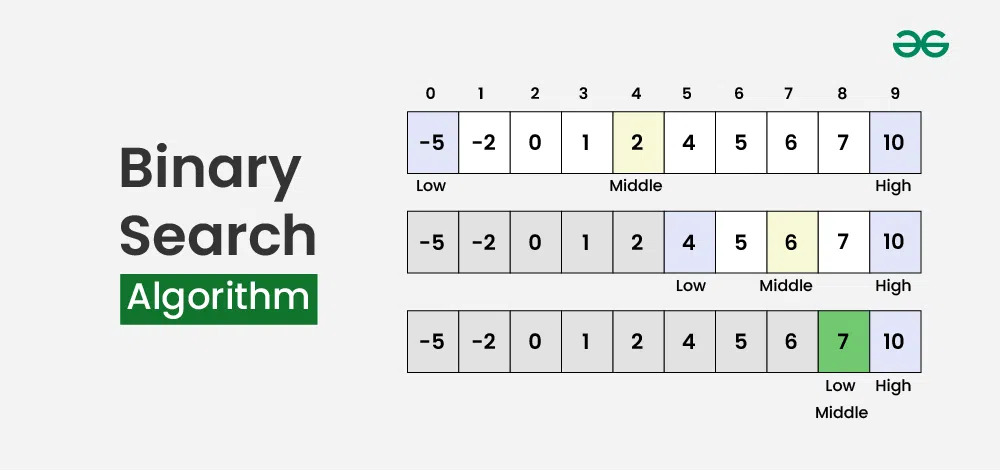
\includegraphics[width=\linewidth,height=6cm,keepaspectratio]{Pictures/ds-algo/binnary-search.jpg}
            \caption{Binary Search Algorithm}
        \end{figure}
    \end{minipage}
    \hfill
    \begin{minipage}[t]{0.55\linewidth}
        \begin{table}[H]
            \begin{tabular}{l l p{4cm}}
                \multicolumn{3}{c}{\textbf{Time Complexity}} \\
                 Best Case & $O(1)$ & \\
                 Average Case & $O(\log(N))$ &  \\
                 Worst Case & $O(\log(N))$ &  \\
                 \multicolumn{3}{c}{\textbf{Space Complexity}}\\
                 Auxiliary Space & $O(1)$ & \\
                 Auxiliary Space & $O(\log(N))$ & recursive call stack \\
            \end{tabular}
        \end{table}
    \end{minipage}
\end{table}


\textbf{Steps}:
\begin{enumerate}
    \item Divide the search space into two halves by finding the middle index “mid”.
    \item Compare the middle element of the search space with the key.
    \item If the key is found at middle element, the process is terminated.
    \item If the key is not found at middle element, choose which half will be used as the next search space.
    \begin{enumerate}
        \item If the key is smaller than the middle element, then the left side is used for next search.
        \item If the key is larger than the middle element, then the right side is used for next search.
    \end{enumerate}
    \item This process is continued until the key is found or the total search space is exhausted.
\end{enumerate}

\begin{table}[h]
    \begin{minipage}[t]{0.48\linewidth}
        \textbf{Advantages}:
        \begin{itemize}
            \item Binary search is faster than linear search, especially for large arrays.
            \item More efficient than other searching algorithms with a similar time complexity, such as interpolation search or exponential search.
            \item Binary search is well-suited for searching large datasets that are stored in external memory, such as on a hard drive or in the cloud.
        \end{itemize}
    \end{minipage}
    \hfill
    \begin{minipage}[t]{0.48\linewidth}
        \textbf{Disadvantages}:
        \begin{itemize}
            \item The array should be \textbf{sorted}.
            \item Binary search requires that the data structure being searched be stored in contiguous memory locations. 
            \item Binary search requires that the elements of the array be comparable, meaning that they must be able to be ordered.
        \end{itemize}
    \end{minipage}
\end{table}

\begin{lstlisting}[language=Python, caption=Binary Search (iterative) - Python]
def binarySearch(arr: list, low: int, high: int, x: object):
    while low <= high:
        mid = low + (high - low) // 2

        # Check if x is present at mid
        if arr[mid] == x: return mid

        # If x is greater, ignore left half
        elif arr[mid] < x: low = mid + 1

        # If x is smaller, ignore right half
        else: high = mid - 1

    # If we reach here, then the element was not present
    return -1
\end{lstlisting}

\begin{lstlisting}[language=Python, caption=Binary Search (recursive) - Python]
def binarySearch(arr: list, low: int, high: int, x: object):
    # Check base case
    if high >= low:
        mid = low + (high - low) // 2
        
        # If element is present at the middle itself
        if arr[mid] == x: return mid
            
        # If element is smaller than mid, then it
        # can only be present in left subarray
        elif arr[mid] > x: 
            return binarySearch(arr, low, mid-1, x)

        # Else the element can only be 
        # present in right subarray
        else: return binarySearch(arr, mid + 1, high, x)

    # Element is not present in the array
    else: return -1
\end{lstlisting}








































